%\documentclass[10pt,t]{beamer}
%\documentclass[t,serif]{beamer}
%\documentclass[10pt,t,handout,serif,professionalfont]{beamer}
%\documentclass[11pt,t,serif,professionalfont,xcolor={dvipsnames}]{beamer}
\documentclass[%
% handout,% comment out for overlays
    slidestop,%
    compress,%
    mathserif,%
    table,%
    usenames,%
    aspectratio=169,
    dvipsnames,%
%noamsthm
]{beamer}%
%\documentclass[t,serif]{beamer}
%\setbeameroption{show notes}
%\setbeameroption{show only notes}

%%%% Notes on the second screen
%\usepackage{pgfpages}
%\setbeameroption{show notes on second screen}

\usepackage{main}
\usepackage{fzeyda}
%\usepackage{rye}

%%%%%%%%%%%%%%%%%%%%%%%%%%%%%%%%%%%%%%%%%%%%%%%%%%%%%%%%%%%%%%%%%%%%%%%%%%
% From RoboStar beamer template
%%%%%%%%%%%%%%%%%%%%%%%%%%%%%%%%%%%%%%%%%%%%%%%%%%%%%%%%%%%%%%%%%%%%%%%%%%

\mode<presentation>{
    \usetheme[compress]{Dresden}
    \definecolor{beamer@header}{HTML}{666666}
    \definecolor{beamer@blendedblue}{HTML}{015580}
    \definecolor{beamer@line}{HTML}{b5c55c}
    \definecolor{beamer@zed}{HTML}{0172ac}
    \definecolor{beamer@orange}{HTML}{ff4000}
    \setbeamercolor*{palette primary}{fg=white,bg=beamer@header}
    \setbeamercolor*{palette secondary}{fg=white,bg=beamer@line}

    \setbeamercolor{frametitle}{fg=beamer@blendedblue,bg=gray!10!white}
    \setbeamercolor{structure}{fg=beamer@header}
    \setbeamercolor{titlelike}{parent=palette primary,bg=white,fg=beamer@blendedblue}
    \setbeamercolor{navigation symbols}{fg=beamer@line, bg=beamer@header}
    \setbeamertemplate{page number in head/foot}[totalframenumber]
    % \expandafter\def\expandafter\insertshorttitle\expandafter{%
    %     \insertshorttitle\hfill%
    % \hfill\hspace{8cm}\insertframenumber\,/\,\inserttotalframenumber}
    % Comment the line below if you want to use the navigation symbols.
    \beamertemplatenavigationsymbolsempty
}

\settowidth{\leftmargini}{\usebeamertemplate{itemize item}}
\addtolength{\leftmargini}{\labelsep}
\setbeamerfont{caption}{size=\scriptsize}
\setbeamertemplate{footline}[frame number]

\defbeamertemplate*{title page}{customized}[1][]
{
    \centering
    \vspace{1em}
    {\usebeamerfont{title}\usebeamercolor[fg]{frametitle}\inserttitle}\par
    \vspace{1em}
    {\usebeamerfont{subtitle}\usebeamercolor[fg]{subtitle}\insertsubtitle}\par
    \bigskip
    {\usebeamerfont{author}\usebeamercolor{titlelike}\insertauthor}\par
    \bigskip
    \vspace{1em}
    
\includegraphics[scale=0.18]{pics/RoboStar_FC.eps}\par
    \vspace{0.5em}
    {\small \href{https://robostar.cs.york.ac.uk/}{robostar.cs.york.ac.uk}}\par
    \vspace{1em}
    {\tiny \usebeamerfont{date}\insertdate}\par
    \usebeamercolor[fg]{titlegraphic}\inserttitlegraphic
}

\setbeamertemplate{headline}
 {%
   %\begin{beamercolorbox}[colsep=1.5pt]{upper separation line head}
   %\end{beamercolorbox}
   \begin{beamercolorbox}[ht=5.5ex]{section in head/foot}
     \vskip1pt\insertnavigation{\paperwidth}\vskip2pt
   \end{beamercolorbox}%
 % \ifbeamer@theme@subsection%
     \begin{beamercolorbox}[colsep=1.5pt]{middle separation line head}
     \end{beamercolorbox}
     \begin{beamercolorbox}[ht=0ex,dp=1.125ex,%
       leftskip=.3cm,rightskip=.3cm plus1fil]{subsection in head/foot}
       \usebeamerfont{subsection in head/foot}\insertsubsectionhead
     \end{beamercolorbox}%
 %  \fi%
   \begin{beamercolorbox}[colsep=1.5pt]{lower separation line head}
   \end{beamercolorbox}
}
%\usepackage[color]{circus}

%%%%%%%%%%%%%%%%%%%%%%%%%%%%%%%%%%%%%%%%%%%%%%%%%%%%%%%%%%%%%%%%%%%%%%%%%%
%%%%%%%%%%%%%%%%%%%%%%%%%%%%%%%%%%%%%%%%%%%%%%%%%%%%%%%%%%%%%%%%%%%%%%%%%%

% reduce margin
\setbeamersize{text margin left=0.4cm,text margin right=0.4cm} 

%%%%%%%%%%%%%%%%%%%%%%%%%%%%%%%%%%%%%%%%%%
% Body 
%%%%%%%%%%%%%%%%%%%%%%%%%%%%%%%%%%%%%%%%%%
%\title[Automated Reasoning of Probabilistic Programs]{
%	Automated Reasoning for Probabilistic Sequential Programs\\ with Theorem Proving
%}
%\author[K. Ye, S. Foster, J. Woodcock]{\underline{Kangfeng Ye}, Simon Foster, Jim Woodcock}
%\institute[UoY]{\normalsize RoboStar\footnotemark[1]}

%\date{November 04, 2021}

%\titlegraphic{
\includegraphics[align=c,width=4.2cm]{pics/UOY-Logo}\qquad
\includegraphics[align=c,width=5.6cm]{pics/EPSRC_logo}}

\def\Circus{{\sf\slshape Circus}}

\begin{document}

%%%%%%%%%%%%%%%%%%%%%%%%%%%%%%%%%%%%%%%%%%%%%%%%%%%%%%%%%%%%%%%%%%%%%%%%%%%%%%%
%%%%%%%%%%%%%%%%%%%%%%%%%%%%%%%%%%%%%%%%%%%%%%%%%%%%%%%%%%%%%%%%%%%%%%%%%%%%%%%

\title[Programming choices]{{\Large A tour through the programming choices: semantics and applications}}
\subtitle{\large On the occasion of Jim Woodcock's Festschrift}


\author[\underline{Pedro Ribeiro} et al.]
{\normalsize \underline{Pedro Ribeiro}, \underline{Kangfeng Ye}, Frank Zeyda, Alvaro Miyazawa}

%\institute[University of York]{\normalsize University of York, UK}

\date{\small Sept 4, 2024}

%%%%%%%%%%%%%%%%%%%%%%%%%%%%%%%%%%%%%%%%%%%%%%%%%%%%%%%%%%%%%%%%%%%%%%
%%%%%%%%%%%%%%%%%%%%%%%%%%%%%%%%%%%%%%%%%%%%%%%%%%%%%%%%%%%%%%%%%%%%%

\frame{%
    \titlepage
    {%\centering
        %\medskip
        % Here you can include the UoY logo, for example. EPS format will 
        % typically be converted to PDF automatically if using pdflatex.
        %
        %\includegraphics[scale=.04]{pics/UoY-Logo.eps} \qquad
        %\hfill
        % 
\includegraphics[align=c,width=5.6cm]{pics/EPSRC_logo}
        
\includegraphics[align=c,width=2.6cm]{pics/UOY-Logo}
        \hfill\hspace{4cm} 
\includegraphics[align=c,width=3.6cm]{pics/EPSRC_logo}
    }

    %
    % See https://www.york.ac.uk/staff/external-relations/brand/logo/
    % for source of UoY logo.
    % 
    % Include other logos as appropriate.
    %
    %\smallskip
    %\href{https://robostar.cs.york.ac.uk}{robostar.cs.york.ac.uk}

}%

\logo{
\includegraphics[scale=0.10]{pics/RoboStar_FC.eps}\quad}

\setbeamerfont{footnote}{size=\tiny}

\begin{frame}{Jim Woodcock}
    \begin{itemize}
        \item This talk is dedicated with affection to Prof. Jim Woodcook on his retirement from University of York.
    \end{itemize}

    % We've all had the pleasure to study and work with Jim for many years.
    % This paper is inspired by Jim's efforts to unify different programming and modelling paradigms.

    \pause \begin{block}{How the authors met Jim}
    \begin{itemize}
        \pause \item Pedro: First heard about the UTP from Jim in the Summer of 2010 while an MEng student at York.
        \pause \item Kangfeng (Randall): Started his PhD at York in 2012 under Jim's supervision, heard and learned Z, CSP, UTP, ... and worked with Jim on a EU project and 4 EPSRC projects.
        \pause \item Frank: First met Jim at ZB in 2002 and helped to run the first UTP symposium in 2006.
        \pause \item Alvaro: First heard Jim's work on "Using Z" during his undergraduate degree, which inspired his interest in formal methods.
    \end{itemize}
    \end{block}

    % \only<2>{
    %     \begin{block}{Frank}
    %         \begin{itemize}
    %             \item First met Jim at ZB 2002
    %             \item Helped to organise the first  Unifying Theories of Programming (UTP) Symposium in 2006
    %             \item Joined Jim and Ana's team at York in 2007 after his PhD
    %             \item Now an independent researcher, living in Mexico 
    %         \end{itemize}
    %     \end{block}
    % }

    % \only<3>{
    %     \begin{block}{Alvaro}
    %         \begin{itemize}
    %             \item First heard Jim's work "Using Z: : Specification, Refinement, and Proof" during his undergraduate degree, which inspired his interest in formal methods
    %             \item Started his PhD study in Jim and Ana's group at York in 2008
    %             \item Continue to work in the Circus and RoboStar groups
    %             \item A lecturer in CS
    %         \end{itemize}
    %     \end{block}
    % }

    % \only<4>{
    %     \begin{block}{Pedro}
    %         \begin{itemize}
    %             \item First heard about UTP as an MEng student at York when attending Jim's lectures in 2010, which had a profound impact on his career
    %             \item Started his PhD study in Angelic processes in 2011, supervised by Prof. Ana Cavalcanti
    %             \item Continue to work in the Circus and RoboStar groups
    %             \item A lecturer in CS
    %         \end{itemize}
    %     \end{block}
    % }

    % \only<5>{
    %     \begin{block}{Kangfeng (Randall)}
    %         \begin{itemize}
    %             \item First met Jim at York in 2012 for his PhD study, supervised by Jim
    %             \item First heard and learned Z, CSP, UTP etc. from Jim
    %             \item Worked with Jim in one EU project and four EPSRC projects in probabilistic semantics for RoboChart
    %             \item A research associate at York, working on formal verification of security protocols  
    %         \end{itemize}
    %     \end{block}
    % }
\end{frame}


\begin{frame}[fragile]
    \frametitle{Outline}
    \setlength{\parskip}{-1ex} %reduce vertical space between entries
    \begin{minipage}{\textwidth} % use minipage to reduce vertical space between entries
        \tableofcontents[hideallsubsections]
    \end{minipage}
\end{frame}

% TOC
%\AtBeginSubsection[]
%\AtBeginSection[]
%{
%  \begin{frame}<beamer>
%    \frametitle{Outline}
%%    \tableofcontents[currentsection,currentsubsection]
%    \tableofcontents[currentsection, hideallsubsections]
%  \end{frame}
%}

% insert a TOC in the beginning of each section
% \AtBeginSection[]
% {
%     \begin{frame}<beamer>
%         \frametitle{Outline}
%         \setlength{\parskip}{-1ex}
%         \begin{minipage}{\textwidth} % use minipage to reduce vertical space between entries
%             \tableofcontents[
%                 currentsection,
%                 hideallsubsections,
%             %currentsubsection, 
%             %hideothersubsections, 
%                 sectionstyle=show/shaded, % current section show and other sections shaded
%                 subsectionstyle=show/shaded/hide, % current section show, other subsections in this section shaded, subsections in other sections hide
%             ] 
%         \end{minipage}
%     \end{frame}
% }

% insert a TOC in the beginning of each subsection
%    \AtBeginSubsection[]
%    {
%        \begin{frame}<beamer>
%            \frametitle{Outline}
%            \tableofcontents[
%        %currentsection,
%        %currentsubsection, 
%        %hideothersubsections, 
%                sectionstyle=show/shaded, % current section show and other sections shaded
%                subsectionstyle=show/shaded/hide,  % current section show, other subsections in this section shaded, subsections in other sections hide
%            ] 
%        \end{frame}
%    }

\section{Motivation and overview}
\begin{frame}{Motivation and overview}
    % more compact and high-level diagram of Fig. 1
    % Applications: FMI, RoboChart
    \begin{columns}%
        \begin{column}[t]{0.55\textwidth}%
            \begin{itemize}%
                \item Review related work in authors' research interests%: semantics for nondeterministic choice, angelic choice, preferential choice, and probabilistic choice in programming
                \item In the context of Jim's research domains%: Z, CSP, Circus, and UTP 
                \item Applications: FMI and RoboChart
                \item Sequential and concurrent programming
            \end{itemize}%
        \end{column}%
        \begin{column}[t]{0.45\textwidth}%
            \begin{center}%
                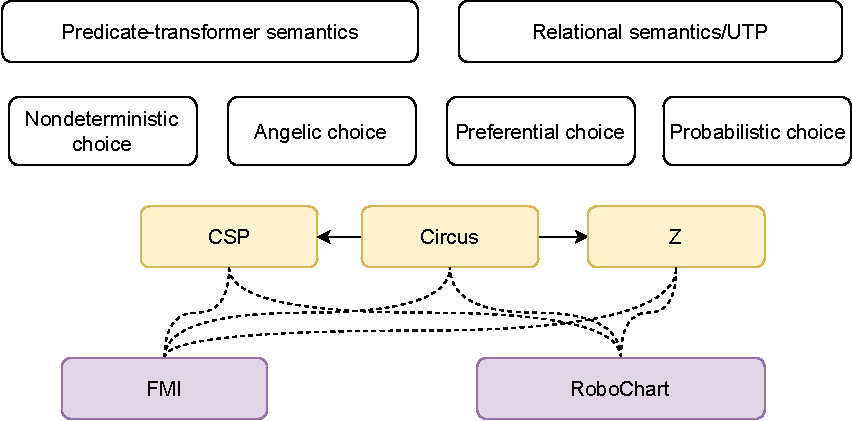
\includegraphics[width=\textwidth]{pics/overall.pdf}%
            \end{center}%
        \end{column}%
    \end{columns}
\end{frame}

\begin{frame}{Informal definitions of various choices}
    \begin{block}{(Demonic) Nondeterministic choice}
        $P \intchoice Q$: choice is resolved in favor of the (worst) undesired result, such as non-termination
    \end{block}
    \begin{block}{Angelic choice}
        $P \sqcup Q$: choice is resolved in favor of the (best) desired result, such as termination
    \end{block}
    \begin{block}{Preferential choice}
        $S \pref T$: behaves like $S$ if $S$ and its continuation is feasible (non-miracle); otherwise, like $T$
    \end{block}
    \begin{block}{Probabilistic choice}
        $P \pchoice{r} Q$: resolved based on the probability $r$ to choose $P$ and $1-r$ to choice $Q$
    \end{block}
    
    \note[item]<1>{We could mention commutative property: Preferential choice is non-commutative and probabilistic choice is quasi-commutative.}
\end{frame}

\section{Nondeterministic choice}
% One slide for each choice and each for application
\begin{frame}{Nondeterministic choice}
    \begin{quote}
        ``A system which permits user programs to become non-deterministic
        presents dreadful problems to the maintenance engineer: it is not a 
        `facility' to be lightly granted.'' \cite[p.12]{EWD:EWD418}, (Hoare quoted by Dijkstra.)%(EWD418, p. 12)
    \end{quote}
    \pause
    \begin{itemize}
        \item Originally not \emph{demonic}\footnote{Dijkstra's allegory of a ``daemon [that] decides quite arbitrarily.''}, as in Rabin and Scott's automata and Turing machines.
        \item McCarthy's $amb$iguity operator.
        \item Dijkstra would embrace it in his GCL after overcoming ``considerable mental resistance'':
            \begin{itemize}
                \item $wp(x:=1 \sqcap x:=2, \{ x = 1 \lor x = 2 \})$, but $wp(..., \{x=1\})$ and $wp(..., \{x=2\})$ not feasible.
                \item By considering conjunctive, rather than arbitrary, predicate transformers, cannot entertain a program that is guaranteed to establish either outcome in isolation.
            \end{itemize}
        \item Contrast with Floyd's choice points, that take the \emph{angelic} view.
    \end{itemize}
\end{frame}

\begin{frame}{Application of nondeterministic choice}
    % maybe discuss the role of non-determinism in RoboChart and the need for the cover wfc and the consequence of removing it.
    \begin{itemize}
        \item Nondeterminism naturally surfaces in theories for refinement, for example, in CSP:
            \begin{displaymath}%
                \begin{aligned}[t]%
                    P_0 &= (e?x \then Skip \extchoice e!0 \then Skip) \lpar \{e\} \rpar e!1 \then Skip = e!1 \then Skip\\
                    P_1 &= (a \then e?x \then Skip \extchoice a \then e!0 \then Skip) \lpar \{e\} \rpar e!1 \then Skip
                \end{aligned}%
            \end{displaymath}\vspace{-2ex}%
        \pause \item Notable laws of programming: 
            \begin{itemize}
                \item $P \sqcap Q \sqsubseteq P$
                \item $P \sqsubseteq Q \iff P = P \sqcap Q$
                \item $\bot \sqcap P = \bot$
            \end{itemize}
        \item CSP processes can be recast as reactive designs in the relational UTP of Hoare and He~\cite{Hoare1998}, where nondeterministic choice is the greatest lower bound of the lattice.
    \end{itemize}
\end{frame}

\section{Angelic choice}
\begin{frame}{Angelic choice}
    \begin{itemize}
        \pause \item Earliest use of the term \emph{angelic} seems due to Broy and Wirsing~\cite{BroyW81}, who studied four types of nondeterminism via algebraic data types.
        \pause \item Hesselink considered extension of GCL with \emph{angelic} choice.
        \pause \item Dijkstra allowed arbitrary predicate transformers for reasoning about UNITY.
        \pause \item Back and von Wright studied sublattices where choice is \emph{angelic} or \emph{demonic}.
        \pause \item As observed by Rewitzky and Brink and others, relations can only capture one type of nondeterminism. Instead, can consider multirelations, i.e. $S \rel \power S$.
        %\item UTP relations, designs, isomorphic to conjunctive monotonic predicate transformers.
        \pause \item Ribeiro and Cavalcanti~\cite{RibeiroC19} encoded binary multirelations in the UTP via non-homogeneous reactive designs to cater for angelic nondeterminism in CSP, where:
            \begin{itemize}
                \pause \item $a \then Skip \sqcup b \then \bot = a \then Skip \sqcup b \then Choice$
                \pause \item $a \then Skip \sqcup b \then \bot = a \then Skip$ (when preservation of trace history is relaxed)
            \end{itemize}
    \end{itemize}
\end{frame}

\begin{frame}{Application of angelic choice}
    \begin{itemize}
        \pause \item Several applications in the literature, mainly in sequential programming: data refinement, proof tactics, constraint and logic programming, modelling games, conformance relations.
        \pause \item Co-simulation master algorithm in FMI: 
            \begin{itemize}
                \pause \item FMUs may refuse to step their simulation by a given step size.
                \pause \item Master algorithm can backtrack the simulation by restoring FMU state and trying again.
                \pause \item Goal is to step through the simulation by the largest step accepted by all FMUs.
                \pause \item Paper sketches a \Circus~specification using \emph{angelic} and \emph{demonic} choices.
            \end{itemize}
        \pause \item RoboChart:
            \begin{itemize}
                \pause \item The guards on transitions out of a junction must form a cover.
                \pause \item Such well-formedness condition may be inconvenient.
                \pause \item Alternatively could consider angelic choice over transitions out of a state. If a junction is reached where no guard is true backtracking would enable an alternative path to be taken.
            \end{itemize}
    \end{itemize}
\end{frame}

\section{Preferential choice}
\begin{frame}{Preferential choice $S \pref T$}
    \begin{itemize}
        \only<1->{\item Not commutative and non-monotonic in its first operand,}
        \only<2->{\item Cannot be expressed in wp predicate transformers,}
        \only<3->{\item Prospective values (PV) semantics~\cite{Stoddart2024},} 
        \only<4->{\item Preference in wp: three-valued G\"{o}del logic~\cite{GoedelLogic} (false, true, supertrue), mechanised in Isabelle/HOL (wpe semantics of GCL), including angelic choice} 
        %\only<5->{\item Preference in UTP: future work} 
    \end{itemize}
%
    \only<1>{
        \begin{block}{Non-monotonic}
            \begin{align*}
                & (\alert{x := 1} \pref x := 2) \seqc (x = 1 \precond \gclskip) \textcolor{gray}{\qquad= (x := 1)}\\
                & \not \refinedby \\
                & (\alert{\magic} \pref x := 2) \seqc (x = 1 \precond \gclskip) \textcolor{gray}{\qquad= abort}
            \end{align*}
        \end{block}
    }
%
    \only<2>{
        \begin{block}{wp}
            The closest one in wp is Nelson's biased choices~\cite{Nelson1989}: 
            \[ S \biasedchoice T \deq S \choice \lnot \fis(S) \guards T \]
            but no continuation in biased choice. 
            %Expect 
            %\[\alert{S \choice T} \; \; \refby \; \; S \pref T \; \; \refby \; \; \alert{S \biasedchoice T}\] 
            %in wp, but $S \pref T$ cannot be expressed in wp
        \end{block}
    }

    \only<3>{
        \begin{block}{PV semantics}
            Based on expression transformers~\cite{bGSL2023}: $\alert{S \diamond E}$ (prospective values of expression $E$ after the execution of $S$)\par
            Defined on Hehner's bunch theory:
            \[ (S \pref T) \diamond E \deq (S \diamond E) \bunchcomma (S \diamond E) = \nullbunch \bguards T \diamond E \]
            With nondeterministic choice and probabilistic choice, but without angelic choice
        \end{block}
        \note[item]<3>{Why bunch theory? why no angelic choice?}
    }
\end{frame}

\begin{frame}{Application of preferential choice}
    \begin{itemize}
        \item Semantics of backtracking search algorithms for formal verification: ordered choices
        \item Co-Simulation master algorithm (MA) for FMI: 
            \[ (stepsize := 4 \pref stepsize := 2 \pref stepsize := 1) \seqc (FMU_1 \parc FMU_2 \parc \cdots) \]
    \end{itemize}
\end{frame}

\section{Probabilistic choice}
\begin{frame}{Probabilistic choice $P \pchoice{r} Q$}
    Imperative sequential programming
    \begin{itemize}
        \only<1->{\item Kozen's seminal work~\cite{Kozen1981}: no nondeterministic choice,}
        \only<2->{\item McIver and Morgan's expectation transformer semantics~\cite{McIver2005bn}\only<2>{: nondeterministic choice is the smaller pre-expectation (demonic),}}
        \only<3->{\item He et al.'s "weakest completion"~\cite{He2004} - probabilistic designs,} 
        \only<4->{\item Hehner’s Probabilistic Predicative Programming (PPP)~\cite{Hehner2004} and ProbURel~\cite{Ye2023}} 
    \end{itemize}
    
    \note[item]<1>{Partial measurable functions on a measurable space and continuous linear operators on a Banach space}
    \note[item]<2>{Greatest pre-expectation}
    \note[item]<3>{A design is H3 (its precondition is a condition, won't mention after-state variables) for embedded into probabilistic designs; Sequential composition requires finite state space; Probabilistic choice is not idempotent; }
    \note[item]<4>{Bayesian subjective view}
    \only<5->{
        Concurrent programming (probabilistic process algebras)
        \begin{itemize}
            \only<5->{\item Hansson’s alternating model~\cite{Hansson1991}, Segala and Lynch’s probabilistic automata~\cite{Segala1995}, Van Glabbeek et al.’s reactive, generative, and stratified models~\cite{Vanglabbeek1995}, CSP extensions~\cite{Morgan1996a,Morgan2005,Nunez1995,Gomez1997,Kwiatkowska1998,Sun2010,Georgievska2012}} 
            \only<6->{\item Probabilistic semantics of RoboChart in PRISM~\cite{Ye2022}} 
        \end{itemize}
    }
    \note[item]<5>{Hansson: ; PA: a distribution from a source state may contain more than one action; if only one action, called \alert{simple} PA; }
    \note[item]<5>{Van Glabbeek et al. reactive, generative, and stratified models. \alert{Multiple actions} can be offered by a process to its environment, but the environment is allowed to choose \alert{only one} in the \alert{reactive} model or \alert{some} in the generative and stratified models. After actions are chosen by the environment, the process makes an \alert{internal transition} based on the current state and (1) the probability distribution associated with the action in the reactive model, or (2) the globally (or locally) redistributed probability distribution for chosen actions in the generative (or the stratified) model.}
    \note[item]<6>{CSP extensions: Seidel, Lowe (DTCSP and PDTCSP, no internal nondeterministic choice), Gomez (no internal nondeterministic choice, two versions of probabilistic choices: generative and reactive), Morgan and McIver (PCSP, internal choice is not idempotent), Mislove (extend PCSP to have both nondeterministic choice and probabilistic choice, and nondeterministic choice is idempotent), Georgievska (a probabilistic extension of CSP which preserves the distributivity laws and the idempotent law for internal non- deterministic choice, via restricted schedulers) }
    \note[item]<6>{Sun (PCSP$\#$): MDP, PAT}
    \note[item]<6>{PRISM: MDP}
%
    \only<1>{
    }
%
    \only<2>{
    }

    \only<3>{
        \begin{block}{Probabilistic designs}
            \begin{itemize}
                \item Weakest prespecification~\cite{Hoare1987}
                \item UTP relations with a variable $prob$
                \item Nondeterministic choice and probabilistic choice: refinement
                \item Woodcock et al.~\cite{Woodcock2019} formalised its semantics, and Ye et al.~\cite{Ye2021} mechanised it in Isabelle/UTP,
                \item Probabilistic semantics for RoboChart
            \end{itemize}
        \end{block}
    }

    \only<4>{
    %\begin{block}{Probabilistic Unifying Relations (ProbURel)}
        \centering
        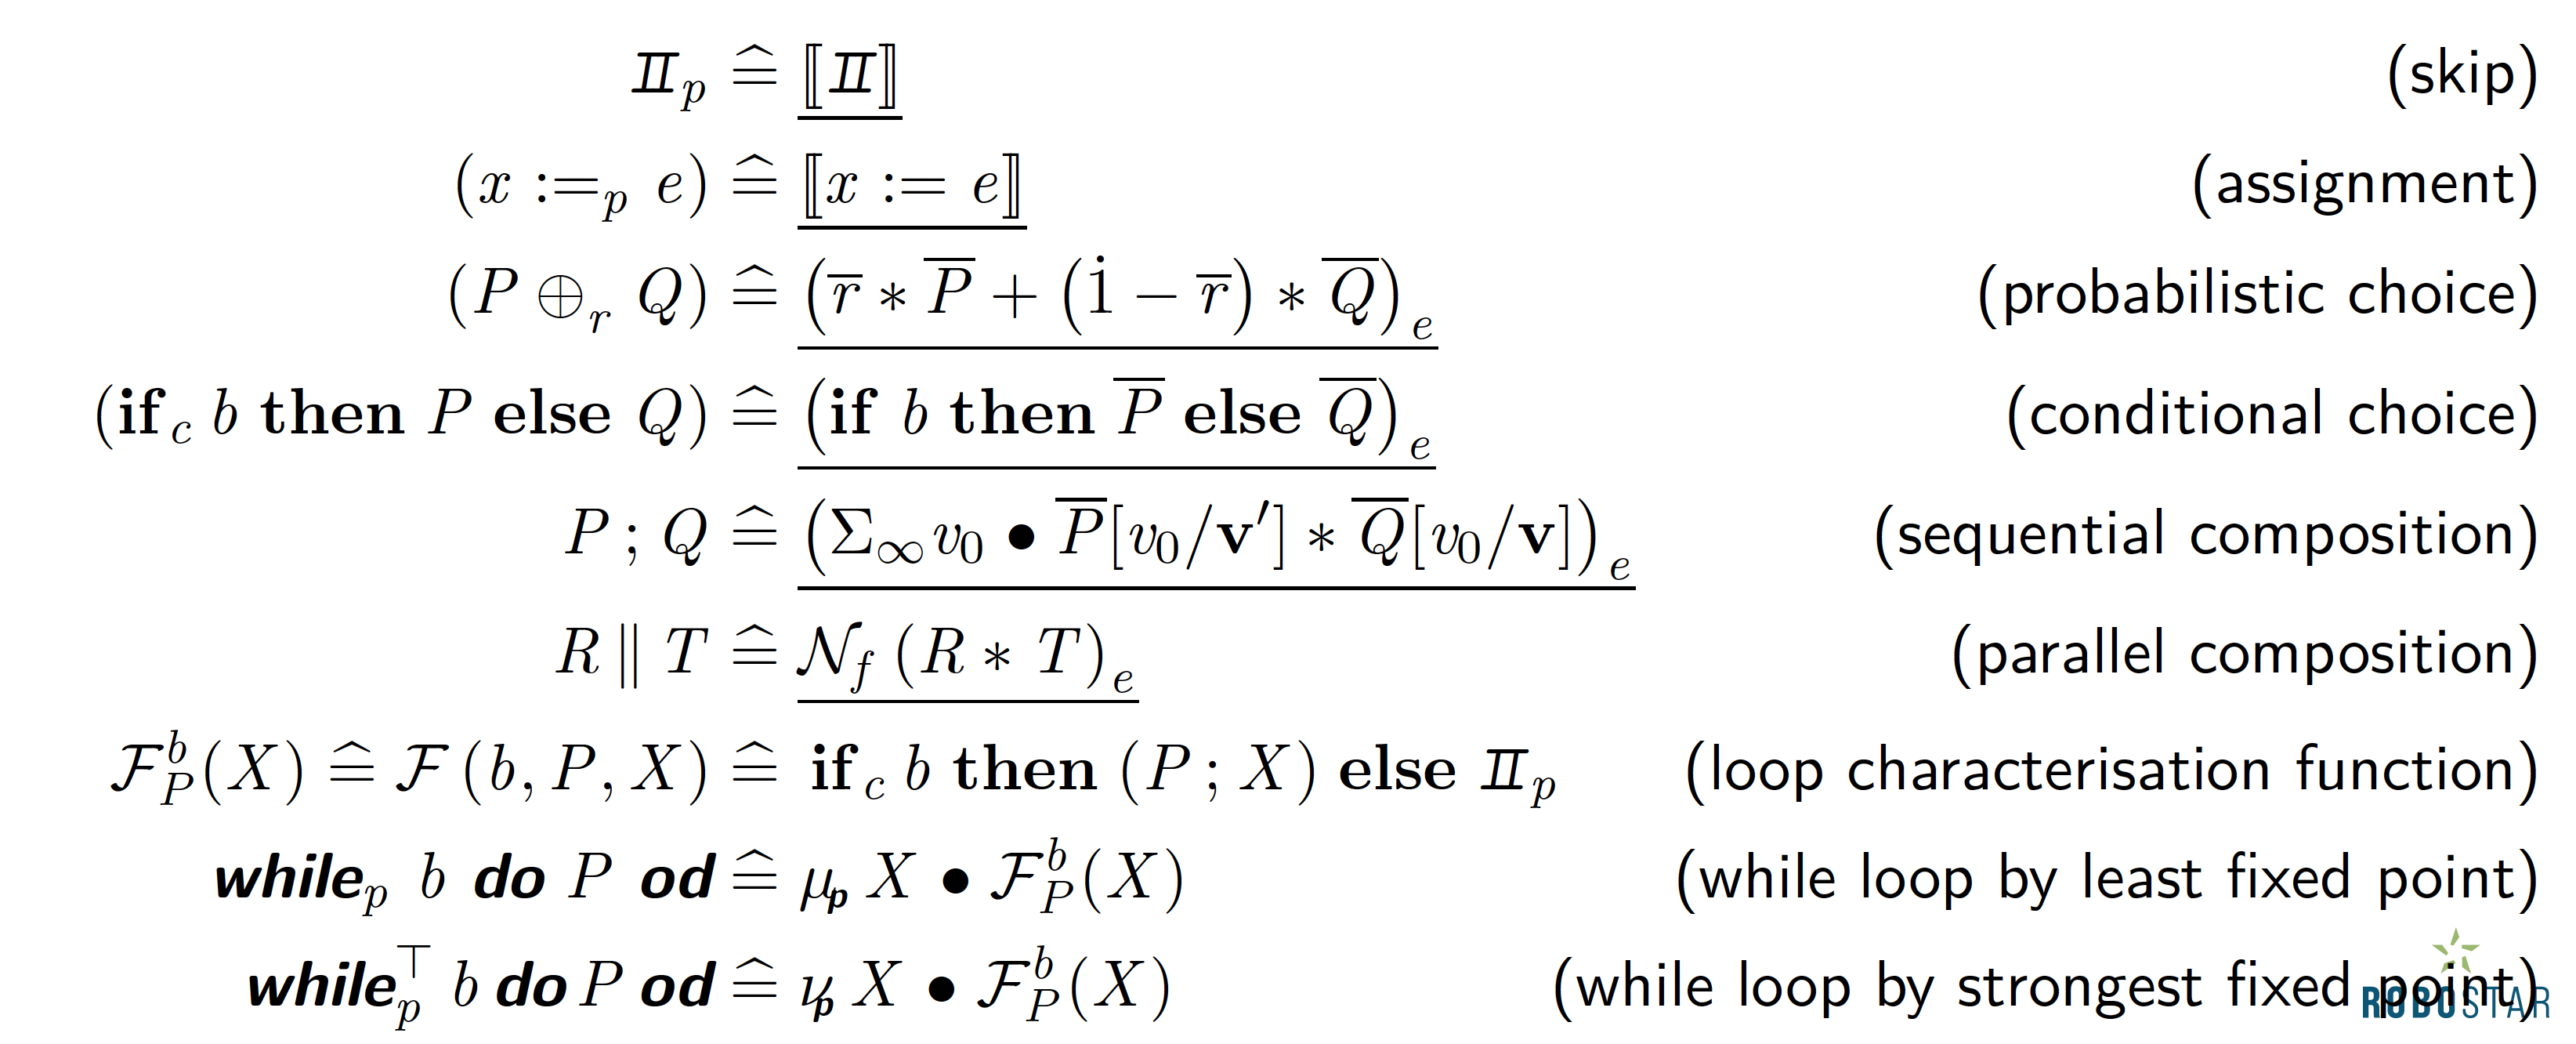
\includegraphics[scale=0.21]{pics/ProbURel.png}
        %\begin{align*}
        %    \pskip & \defs \rvprfunsym{\ibracket{\II}} \tag*{(skip)} \label{def:prog_skip} \\
        %    \left(\passign{x}{e}\right) & \defs \rvprfunsym{\ibracket{x := e}} \tag*{(assignment)} \label{def:prog_assign} \\
        %    \left(\ppchoice{r}{P}{Q}\right) & \defs \rvprfunsym{\usexpr{\prrvfunsym{r} * \prrvfunsym{P} + \left(\rfone - \prrvfunsym{r}\right) * \prrvfunsym{Q}}}\tag*{(probabilistic choice)} \label{def:prog_pchoice} \\ 
        %    \left(\pcchoice{b}{P}{Q}\right)& \defs \rvprfunsym{\usexpr{\IF b \THEN \prrvfunsym{P} \ELSE \prrvfunsym{Q}}}\tag*{(conditional choice)} \label{def:prog_condchoice} \\ 
        %    \pseq{P}{Q} & \defs \rvprfunsym{\usexpr{\infsum v_0 @ \prrvfunsym{P}[v_0/\vv'] * \prrvfunsym{Q}[v_0/\vv]}}\tag*{(sequential composition)} \label{def:prog_seq} \\ 
        %    \pparallel{R}{T} & \defs \rvprfunsym{\normf \usexpr{R * T}}\tag*{(parallel composition)} \label{def:prog_parallel_ff} \\
        %    \lfunbp(X) \defs \lfunp{b}{P}{X} & \defs~\pcchoice{b}{\left(\pseq{P}{X}\right)}{\pskip} \tag*{(loop characterisation function)} \label{def:lfun} \\
        %    \pwhile{b}{P} &\defs \lfp~X @ \lfunbp(X) \tag*{(while loop by least fixed point)} \label{def:pwhile}\\
        %    \pwhiletop{b}{P} &\defs \gfp~X @ \lfunbp(X) \tag*{(while loop by strongest fixed point)} \label{def:pwhile_top}
        %\end{align*}
    %\end{block}
    }
\end{frame}

\begin{frame}[fragile]
    \frametitle{Application of probabilistic choice}
    \only<1>{
        Model epistemic and aleatoric uncertainty and theorem proving~\cite{Ye2023}

        \begin{center}
            $\begin{aligned}
                & CovidTest ::= Pos | Neg \\ 
                & \isakwmaj{alphabet}\ cdstate = c::\bool \quad ct::CovidTest\\
                &Init \defs \left(\ppchoice{p_1}{c := True}{c := False}\right) {\text{\alert{prior}}}\\
                &TestAction \defs \pcchoice{c}
                {(\ppchoice{p_2}{\passign{ct}{Pos}}{\passign{ct}{Neg}})}
                {(\ppchoice{p_3}{\passign{ct}{Pos}}{\passign{ct}{Neg}})} \\
                & FirstTestPos \defs \pparallel{\left(\pseq{Init}{TestAction}\right)}{\ibracket{ct' = Pos}} \\
                &SecondTestPos \defs \pparallel{\left(\pseq{FirstTestPos}{TestAction}\right)}{\ibracket{ct' = Pos}}
            \end{aligned}$
        \end{center}

        Imperfect test: \alert{sensitivity} and \alert{specificity}

       Do we need the 2nd test? How much can it contribute?

       Provided $p_1=0.002$, $p_2=0.89$, and $p_3=0.05$, (38.84\% vs. 3.44\%)
    }
    \only<2->{
        Simple random walk
        \only<2->{
        \begin{center}
            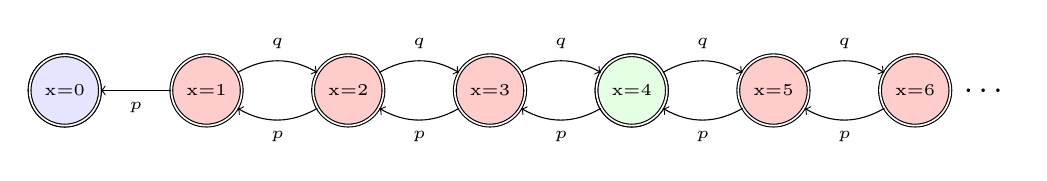
\begin{tikzpicture}[scale=1.2,every node/.style={scale=1.2}]

                \def \n {6}
                \def \margin {8} % margin in angles, depends on the radius
                \def \scale {1.5}
                \def \p {p}
                \def \q {q}

                \foreach \s in {0,...,\n}
                {
                    \node[draw, circle, double, fill=red!20] at (\s*\scale,0) (N\s) {{\tiny x=\s}};
                }

                \node[draw, circle, double, fill=green!10] at (4*\scale,0) (N4) {{\tiny x=4}};
                \node[draw, circle, double, fill=blue!10] at (0,0) (N0) {{\tiny x=0}};
                \node[] at ({(\n+0.5)*\scale}, 0) {\dots};
                %\node[] at ({(0-0.5)*\scale}, 0) {\dots};

                \newcommand{\plusmacro}{%0/1/0/1/1/3, 
                1/2/p/1/2, 2/3/p/1/2, 3/4/p/1/2, 4/5/p/1/2, 5/6/p/1/2}
                \foreach \x/\y/\p\prd/\prm in \plusmacro
                {
                    \path[->] (N\x) edge [bend left] node [above] %{\tiny \{$\frac{\pld}{\plm}$\}:x+1}
                    {\tiny $\q$}
                    (N\y);
                    \path[->] (N\y) edge [bend left] node [below] %{\tiny \{$\frac{\prd}{\prm}$\}:x-1}
                    {\tiny $\p$}
                    (N\x);
                }

                \path[->] (N1) edge node [below] {\tiny $\p$} (N0);

            \end{tikzpicture}
        \end{center}
        }

        % \only<3>{%\Large
        %     %\begin{columns}
        %     %        \begin{column}{0.25\textwidth}
        %     %            \centering
        %     %            Probability theory 
        %     %        \end{column}
        %     %        \begin{column}{0.75\textwidth}
        %     Probability theory
        %     \begin{itemize}
        %         \item $\sigma(m)$: $m$ copies of one-step random walk $\sigma(1)$ 
        %         \item $G_{\sigma(m)}(z)=G_{\sum_{i=0}^{m} \sigma(1)}(z)=\left(G_{\sigma(1)}(z)\right)^m= 
        %             \left(\sum_{n=0}^{\infty} \varphi(n) z^n\right)^m$
        %         \item Condition the first step and solve an equation to get $G_{\sigma(1)}(z)$
        %         \item Taylor expansion to get the distribution $\varphi(n)$
        %     \end{itemize}
        %     %        \end{column}
        %     %    \end{columns}
        % }

        \only<2->{%\Large
            \begin{columns}
                \begin{column}{0.30\textwidth}
                    \vspace*{-2em}
                    \centering
                    \begin{align*}
                        &x := m; t:=0; \\
                        &\text{while}(x > 0) \{\\
                            &\quad {\clz x := x - 1 \pchoice{p} x := x + 1 ; }\\
                            &\quad t:=t+1\\
                        &\} 
                    \end{align*}
                \end{column}
                \begin{column}{0.70\textwidth}
                    %\centering
                    \vspace*{-2em}
                    \begin{align*}
                        \only<2>{&\cle \ibracket{\lnot x> 0}*\ibracket{x'=x}*\ibracket{t'=t}+ \\} 
                        \only<3->{&\ibracket{\lnot x> 0}*\ibracket{x'=x}*\ibracket{t'=t} + \\}
                        &\ibracket{x > 0}*\ibracket{x'=0} * \\
                        &\left(
                        \begin{array}[]{l}
                            \only<3>{\cle \ibracket{t'-t\geq x}*\ibracket{((t'-t)-x)\%2=0}*\\
                                \cle \quad\mu(x-1, t'-t-1)*p +\\} 
                            \only<2,4->{\ibracket{t'-t\geq x}*\ibracket{((t'-t)-x)\%2=0}*\\
                                \quad\mu(x-1, t'-t-1)*p +\\} 
                            \only<2-3,5->{\ibracket{t'-t\geq x+2}*\ibracket{((t'-t)-(x+2))\%2=0}*\\
                                \quad\mu(x+1, t'-t-1)*q}
                            \only<4>{\cle \ibracket{t'-t\geq x+2}*\ibracket{((t'-t)-(x+2))\%2=0}*\\
                                \cle \quad\mu(x+1, t'-t-1)*q}
                        \end{array}\right) \\
                        \only<2-4>{&\mu(m, n) = p*\mu(m-1,n-1) + q*\mu(m+1,n-1)}
                        \only<5>{&\cle \mu(m, n) = p*\mu(m-1,n-1) + q*\mu(m+1,n-1)}
                    \end{align*}
                \end{column}
            \end{columns}
        }

        %\only<3>{\large
        %    %\vspace*{-1em}
        %    ProbURel: semantics for the while loop
        %    \begin{align*}
        %        Ht \defs~ &\ibracket{\lnot x> 0}*\ibracket{x'=x}*\ibracket{t'=t} + \\
        %        &\ibracket{x > 0}*\ibracket{x'=0} * \\
        %        &\left(
        %        \begin{array}[]{l}
        %            \ibracket{t'-t\geq x}*\ibracket{((t'-t)-x)\%2=0}*\mu(x-1, t'-t-1)*p +\\ 
        %            \ibracket{t'-t\geq x+2}*\ibracket{((t'-t)-(x+2))\%2=0}*\mu(x+1, t'-t-1)*q
        %        \end{array}\right) \\
        %        \mu(m, n&) = p*\mu(m-1,n-1) + q*\mu(m+1,n-1) \\
        %    \end{align*}
        %}
    }
\end{frame}
% \begin{frame}{Probabilistic choice}
%     \only<1>{
%         %        \begin{center}
%         %            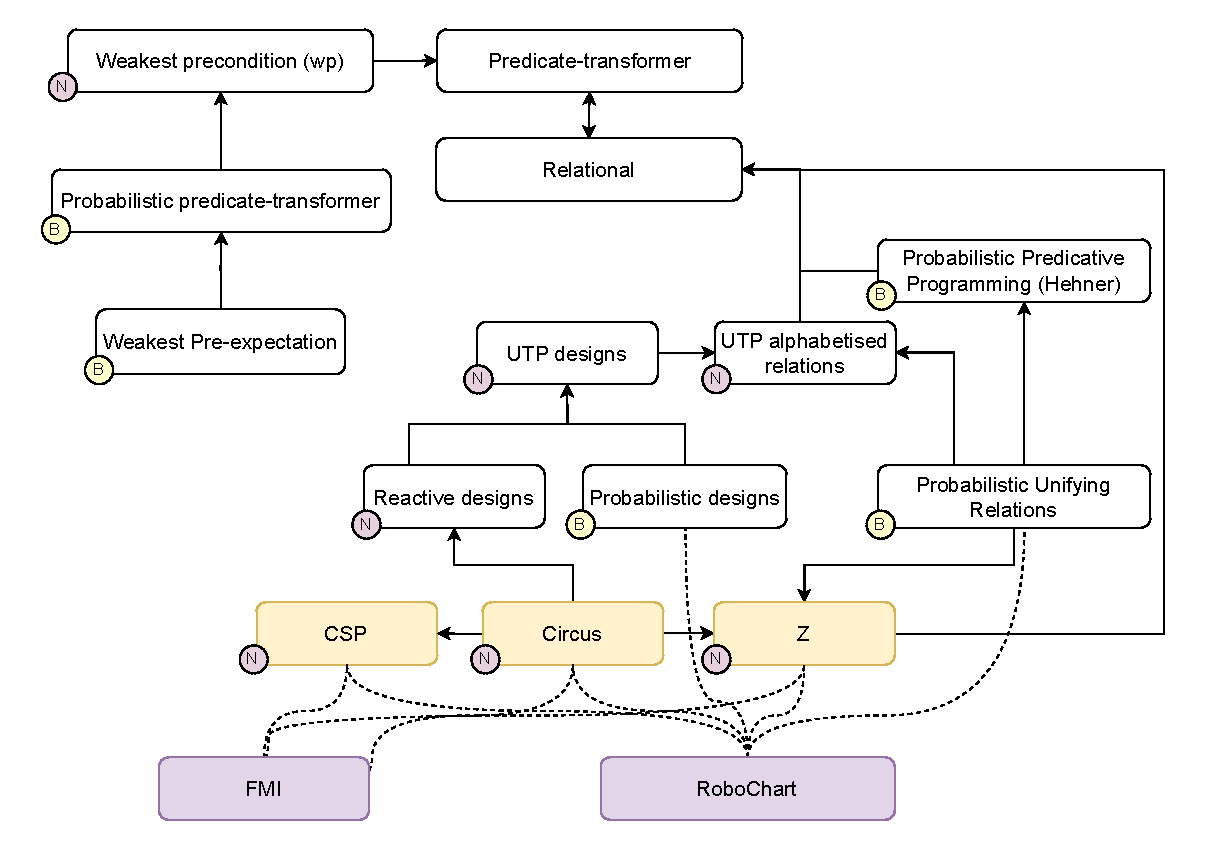
\includegraphics[scale=0.40]{pics/choices-probabilistic.pdf}
%         %        \end{center}
%         %    }
%         %        \only<1>{
%         \begin{columns}%
%             \begin{column}[t]{0.5\textwidth}%
%                 \only<1>{Imperative probabilistic %programming
%                     \begin{itemize}
%                         \item Kozen's seminal work~\cite{Kozen1981}%: no nondeterministic choice
%                         \item McIver and Morgan's expectation transformer semantics~\cite{McIver2005bn}%: nondeterministic choice is the smaller pre-expectation (demonic)  
%                         \item He et al.'s "weakest completion"~\cite{He2004} - probabilistic designs~\cite{Woodcock2019,Ye2021}
%                             \note[item]<2>{Jim et al. formalised the semantics and Ye et al. mechanised in Isabelle/UTP}
%                         \item Hehner’s Probabilistic Predicative Programming (PPP)~\cite{Hehner2004} and ProbURel~\cite{Ye2023}
%                             \note[item]<2>{Ye et al. formalised the semantics using UTP for relations and mechanised in Isabelle/UTP}
%                     \end{itemize} 
%                 }
%             \end{column}
%             \begin{column}[t]{0.5\textwidth}
%                 \vspace*{-2em}
%                 \begin{center}
%                     {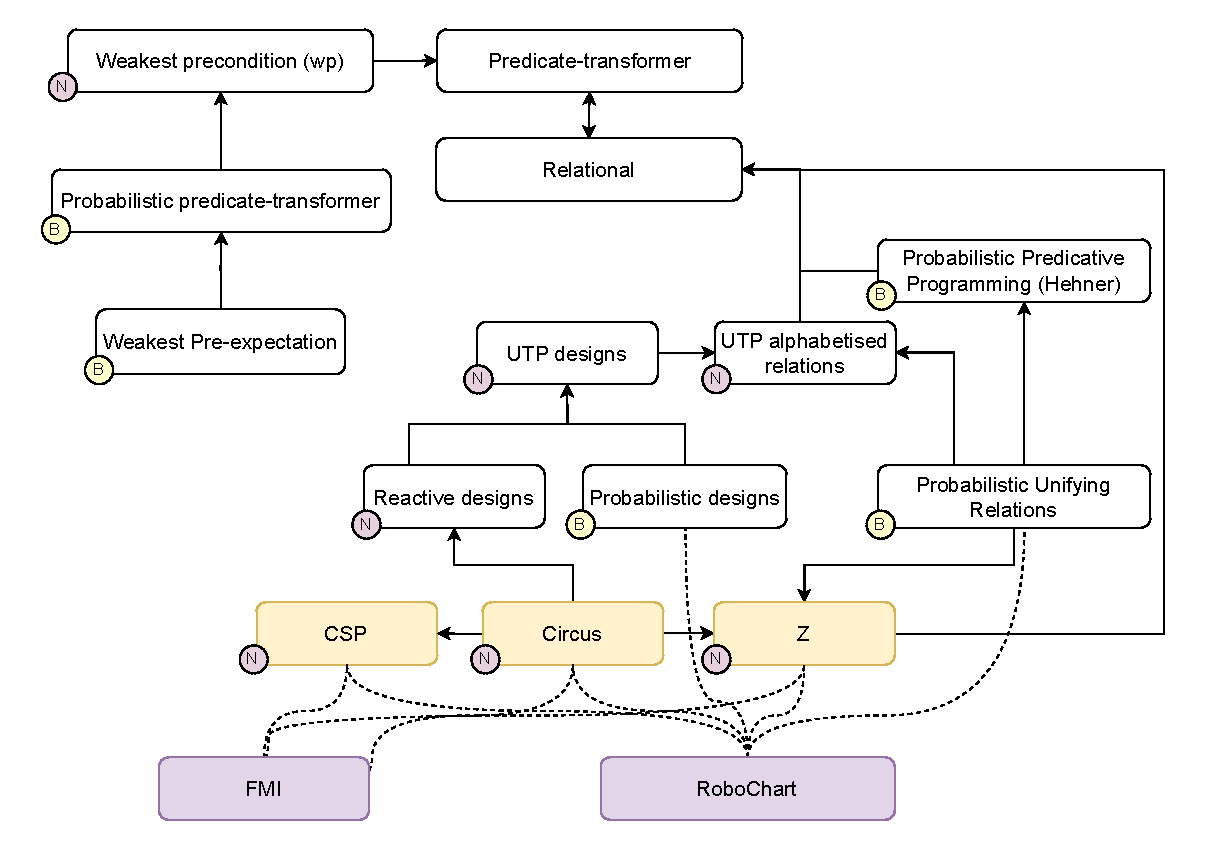
\includegraphics[width=\linewidth]{pics/choices-probabilistic.pdf}}
%                     %\only<3>{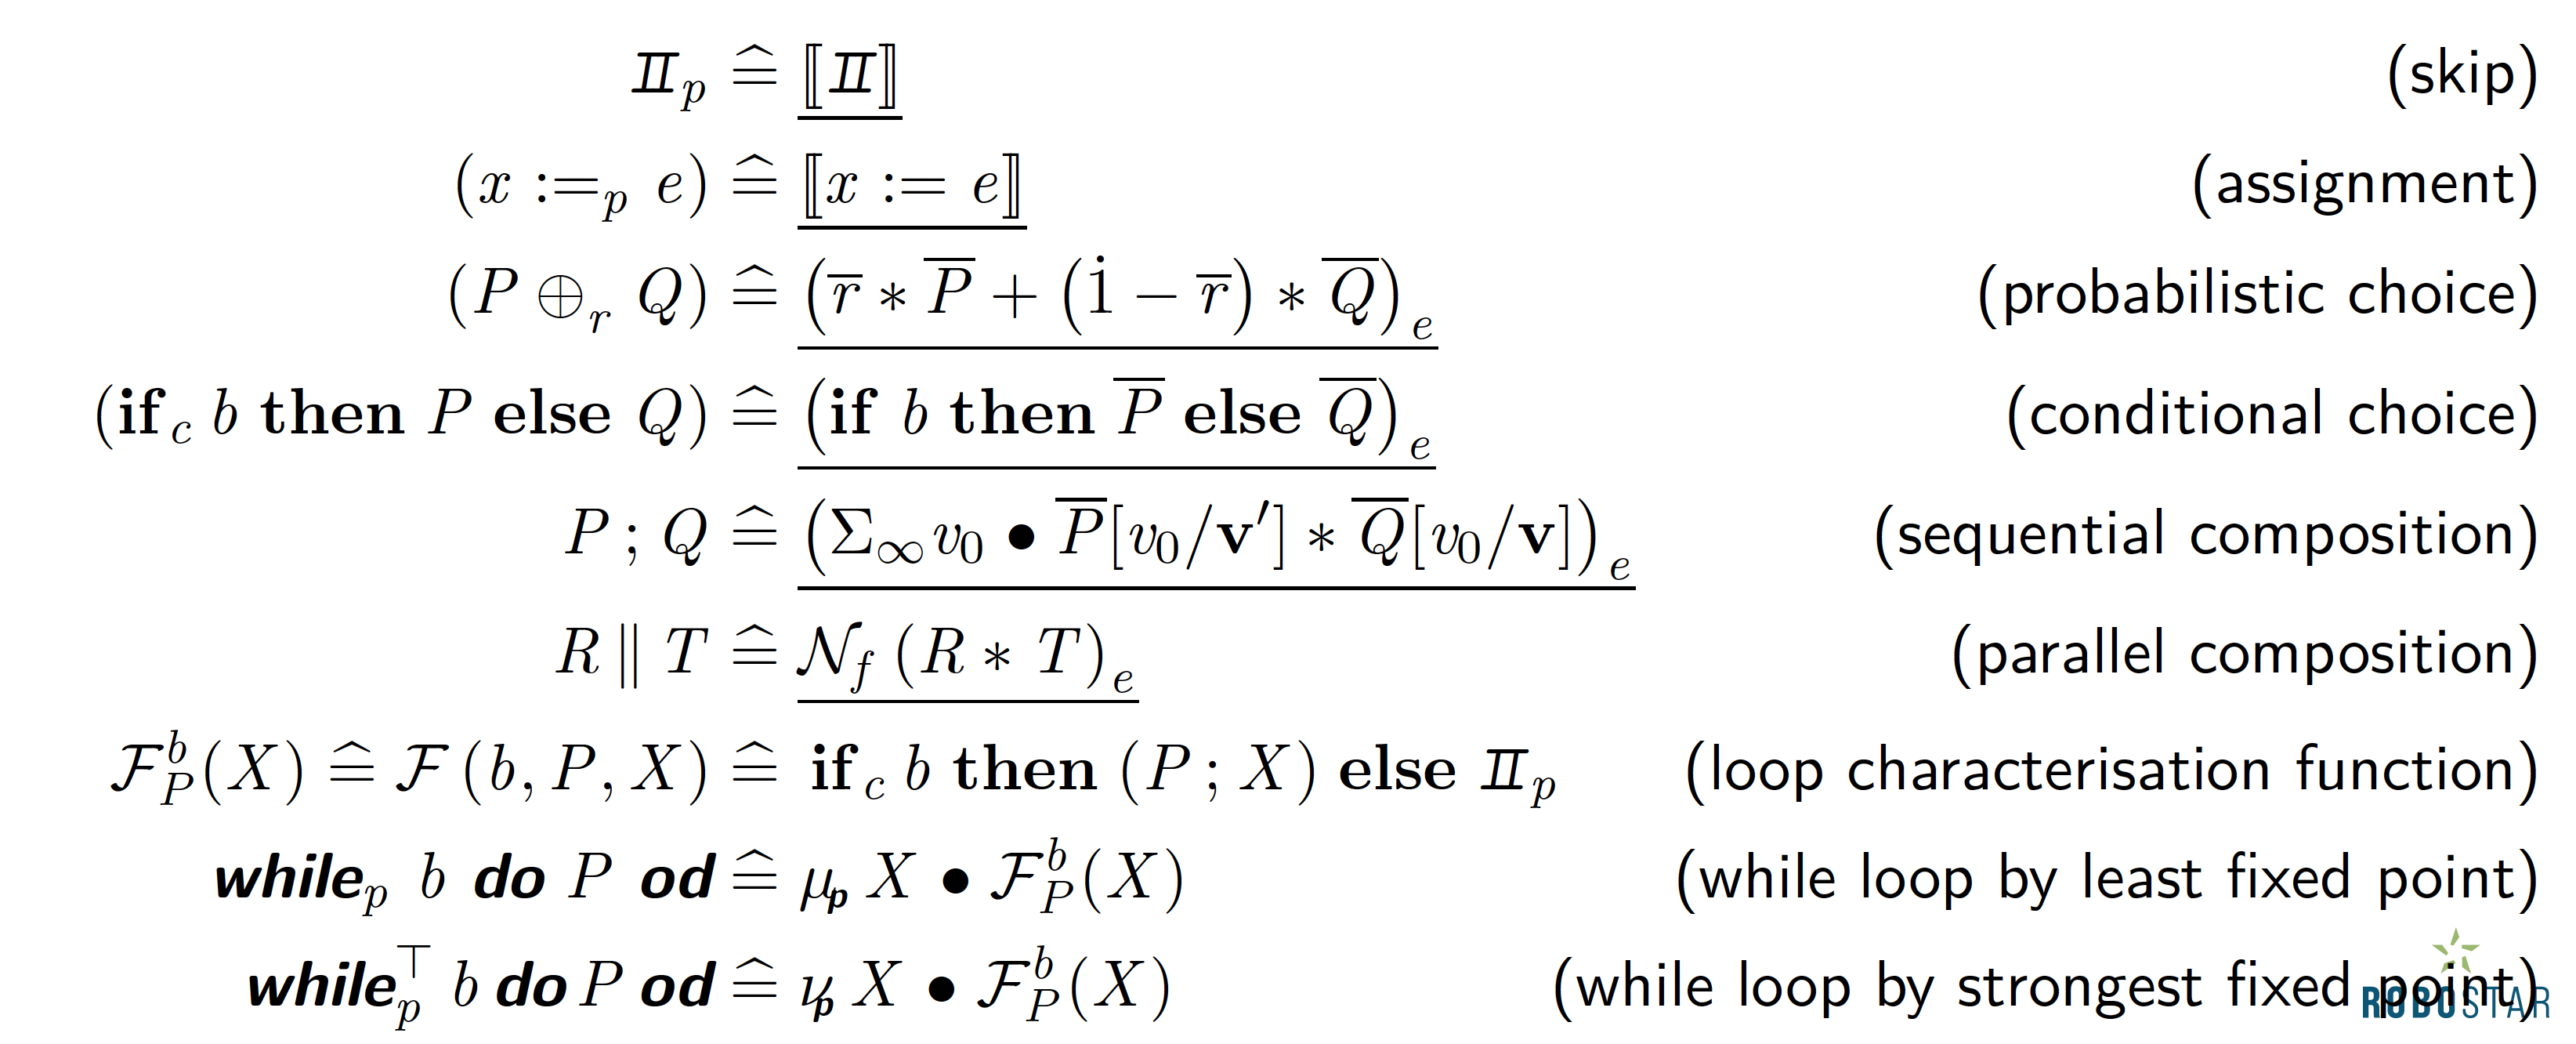
\includegraphics[scale=0.40]{pics/ProbURel.png}}
%                 \end{center}
%             \end{column}
%         \end{columns}
%         \bigskip The support of nondeterministic choice and its interaction with probabilistic choice
%         %{\footnotetext[1]{Kozen, D.: Semantics of probabilistic programs. Journal of Computer and System Sciences 22(3), 328–350 (1981). }}
%     }
%     \only<2>{
%         Probabilistic process algebras
%         \begin{itemize}
%             \item Hansson’s alternating model~\cite{Hansson1991}
%             \item Segala and Lynch’s probabilistic automata~\cite{Segala1995}
%             \item Van Glabbeek et al.’s reactive, generative, and stratified models~\cite{Vanglabbeek1995}
%             \item Probabilistic extensions based on CSP~\cite{Morgan1996a,Morgan2005,Nunez1995,Gomez1997,Kwiatkowska1998,Sun2010,Georgievska2012} 
%             \item Probabilistic semantics of RoboChart in PRISM~\cite{Ye2022} 
%             \note[itemize]<2->{Resolve nondeterministic choice from a state, then probabilistic choice to multiple target states}
%         \end{itemize} \bigskip
%         The support of nondeterministic choice and its interaction with probabilistic choice
%     }
% \end{frame}
% 
% % \begin{frame}[fragile,c]
% %     \frametitle{Probabilistic designs}
% %     \centering
% %     \only<1>{\includegraphics[scale=0.30]{pics/prob_designs.png}}
% % \end{frame}
% 
% \begin{frame}[fragile]
%     \frametitle{Application of probabilistic choice: simple symmetric random walk}
%     \begin{center}
%         \only<1->{
%             \begin{tikzpicture}[scale=1.2,every node/.style={scale=1.2}]
% 
%                 \def \n {6}
%                 \def \margin {8} % margin in angles, depends on the radius
%                 \def \scale {1.5}
%                 \def \p {p}
%                 \def \q {q}
% 
%                 \foreach \s in {0,...,\n}
%                 {
%                     \node[draw, circle, double, fill=red!20] at (\s*\scale,0) (N\s) {{\tiny x=\s}};
%                 }
% 
%                 \node[draw, circle, double, fill=green!10] at (4*\scale,0) (N4) {{\tiny x=4}};
%                 \node[draw, circle, double, fill=blue!10] at (0,0) (N0) {{\tiny x=0}};
%                 \node[] at ({(\n+0.5)*\scale}, 0) {\dots};
%                 %\node[] at ({(0-0.5)*\scale}, 0) {\dots};
% 
%                 \newcommand{\plusmacro}{%0/1/0/1/1/3, 
%                 1/2/p/1/2, 2/3/p/1/2, 3/4/p/1/2, 4/5/p/1/2, 5/6/p/1/2}
%                 \foreach \x/\y/\p\prd/\prm in \plusmacro
%                 {
%                     \path[->] (N\x) edge [bend left] node [above] %{\tiny \{$\frac{\pld}{\plm}$\}:x+1}
%                         {\tiny $\q$}
%                         (N\y);
%                     \path[->] (N\y) edge [bend left] node [below] %{\tiny \{$\frac{\prd}{\prm}$\}:x-1}
%                         {\tiny $\p$}
%                         (N\x);
%                 }
% 
%                 \path[->] (N1) edge node [below] {\tiny $\p$} (N0);
% 
%             \end{tikzpicture}
%         \end{center}
% 
%         \only<2>{%\Large
%             %\begin{columns}
%             %        \begin{column}{0.25\textwidth}
%             %            \centering
%             %            Probability theory 
%             %        \end{column}
%             %        \begin{column}{0.75\textwidth}
%             Probability theory
%             \begin{itemize}
%                 \item $\sigma(m)$: $m$ copies of one-step random walk $\sigma(1)$ 
%                 \item $G_{\sigma(m)}(z)=G_{\sum_{i=0}^{m} \sigma(1)}(z)=\left(G_{\sigma(1)}(z)\right)^m= 
%                     \left(\sum_{n=0}^{\infty} \varphi(n) z^n\right)^m$
%                 \item Condition the first step and solve an equation to get $G_{\sigma(1)}(z)$
%                 \item Taylor expansion to get the distribution $\varphi(n)$
%             \end{itemize}
%             %        \end{column}
%             %    \end{columns}
%         }
% 
%         \only<3>{%\Large
%             \begin{columns}
%                 \begin{column}{0.20\textwidth}
%                     \centering
%                     ProbURel
%                 \end{column}
%                 \begin{column}{0.80\textwidth}
%                     \vspace*{-2em}
%                     \begin{align*}
%                         P \defs \quad & x := m; t:=0; \\
%                                       &\text{while}(x > 0) \{\\
%                                       &\quad {\clz x := x - 1 \pchoice{p} x := x + 1 ; }\\
%                                       &\quad t:=t+1\\
%                                       &\} 
%                     \end{align*}
%                 \end{column}
%             \end{columns}
%         }
% 
%         \only<4>{\large
%             %\vspace*{-1em}
%             ProbURel: semantics for the while loop
%             \begin{align*}
%                 Ht \defs~ &\ibracket{\lnot x> 0}*\ibracket{x'=x}*\ibracket{t'=t} + \\
%                          &\ibracket{x > 0}*\ibracket{x'=0} * \\
%                          &\left(
%                              \begin{array}[]{l}
%                                  \ibracket{t'-t\geq x}*\ibracket{((t'-t)-x)\%2=0}*\mu(x-1, t'-t-1)*p +\\ 
%                                  \ibracket{t'-t\geq x+2}*\ibracket{((t'-t)-(x+2))\%2=0}*\mu(x+1, t'-t-1)*q
%                          \end{array}\right) \\
%                 \mu(m, n) & = p*\mu(m-1,n-1) + q*\mu(m+1,n-1) \\
%             \end{align*}
%         }
%     }
% \end{frame}

\section{Conclusions}
\begin{frame}{Conclusions}
    \only<1>{
    Nondeterministic choice, angelic choice, preferential choice, and probabilistic choice 
    \begin{itemize}
        \item predicate transformers and relational semantics 
        \item in the context of Jim's contributions in CSP, Circus, Z, and UTP
        \item review related work for these choices in sequential and concurrent programming
        \item their applications in FMI and RoboChart
    \end{itemize}
    }

    \only<2>{
    Future work
    \begin{itemize}
        \item Mechanise angelic processes in Isabelle/UTP, explore its refinement laws, and extend with time
        \item Operational semantics for nondeterministic, angelic, and probabilistic choice through Foster's interaction trees~\cite{FosterHW21} for sound animation  
        \item Publish wpe semantics and its mechanisation for preferential choice in wp through three-value logic
        \item Preferential choice in UTP 
        \item Mechanise SRW (with AST and ERT) in Isabelle/UTP, applications (Markov models and Bayesian Networks) and extensions (Nondeterministic choice and concurrency) of ProbURel
    \end{itemize}
    }
\end{frame}

\begin{frame}[c]{ }
    \usebeamerfont{frametitle}\usebeamercolor[fg]{frametitle}
    \centering 
    \Huge
    \emph{Thank you!} \\
    \vspace{0.5em}
    \normalsize
    \color{black}{\href{https://robostar.cs.york.ac.uk/}{robostar.cs.york.ac.uk}}
\end{frame}

%%%% Bibliography %%%%
\newpage
%\bibliographystyle{IEEEtran}
\bibliographystyle{alpha}
\bibliography{main} 
\label{ch:bib} %label to refer to
\end{document}
